
\section*{Question 2}

\subsection*{a) Modifications to General\_polynomial\_itegration.m}

In the uploaded MATLAB tutorial code \texttt{General\_polynomial\_itegration.m}, the original implementation for computing the coefficients of the nth-order polynomial used manual calculations. However, in order to simplify the code and improve efficiency, the \texttt{polyfit} function was introduced. This function fits a polynomial of specified degree to a set of data points using the method of least squares. By using \texttt{polyfit}, we can directly obtain the coefficients vector needed for the nth-order polynomial without manual computation.

The modifications made to the code primarily involve replacing the manual calculation of coefficients with a call to \texttt{polyfit}. Specifically, the lines of code responsible for calculating the coefficients vector have been replaced with a call to \texttt{polyfit}. 

\subsection*{b) Integration of $\frac{\sin(x)}{1+x}$}

Using the modified code, the function $\frac{\sin(x)}{1+x}$ was integrated from 0 to 1 using $n=4$ as the polynomial order and $N=2, 4, 8, 16, 32, 64, 128$ as the number of segments. The true errors for each value of $N$ were tabulated, and a plot of true error vs $N$ was generated. The slope of the plotted curve was determined, indicating the convergence behavior of the numerical integration.

\begin{table}[h]
    \centering
    \begin{tabular}{|c|c|}
    \hline
    $N$ & True Error \\
    \hline
    2 & 6.076888650619061e-07 \\
    4 & 1.15757974872288116330e-08 \\
    8 & 1.92031002210768519944e-10 \\
    16 & 3.04856140331821734435e-12 \\
    32 & 4.77395900588817312382e-14 \\
    64 & 7.21644966006351751275e-16 \\
    128 & 5.55111512312578270212e-17 \\
    \hline
    \end{tabular}
    \caption{True Errors for $\frac{\sin(x)}{1+x}$}
    \label{tab:sinx1plusx}
\end{table}

\clearpage

\begin{figure}[h]
    \centering
    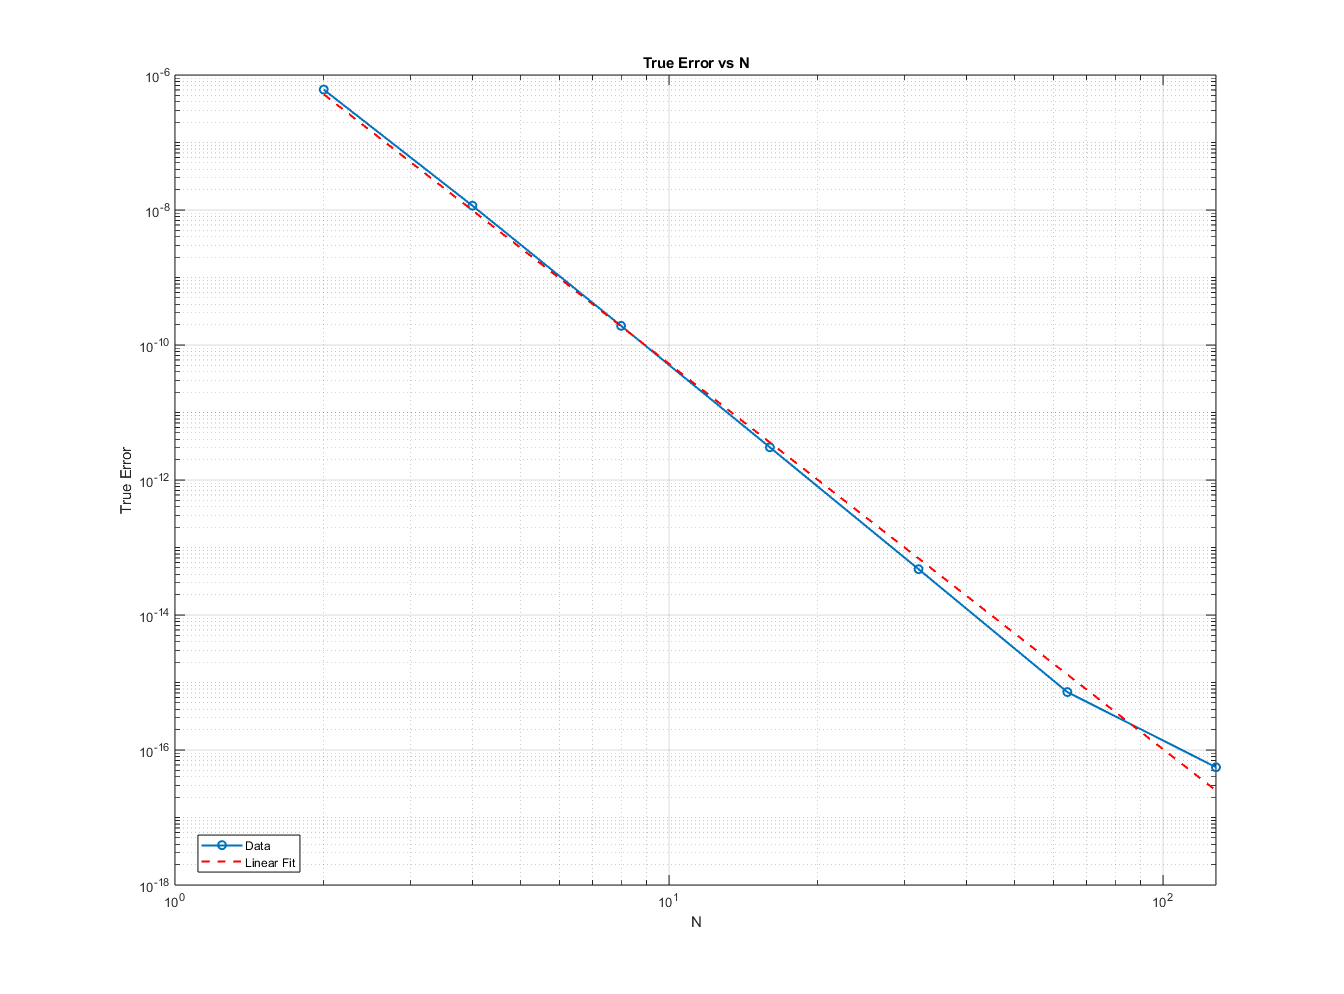
\includegraphics[width=1\textwidth]{Q2-plot1.png}
    \caption{True Error vs $N$ for $\frac{\sin(x)}{1+x}$}
    \label{fig:sinx1plusx}
\end{figure}

The slope of the plotted curve on figure 1 is -5.71, indicating the rate at which the true error decreases with an increase in the number of segments $N$. A steeper negative slope suggests faster convergence, while a shallower negative slope indicates slower convergence.

\subsection*{c) Integration of $\sin(x^3) \cos(x)$}

The integration was repeated for the function $\sin(x^3) \cos(x)$ with limits of integration from 0 to 2.2. The same procedure as in part (b) was followed to obtain the true errors for different values of $N$, and a plot of true error vs $N$ was generated.

\clearpage

\begin{table}[h]
    \centering
    \begin{tabular}{|c|c|}
    \hline
    $N$ & True Error \\
    \hline
    2 & 4.74167945015147029864e-04 \\
    4 & 3.76453500236517690780e-06 \\
    8 & 5.15717486493372234690e-08 \\
    16 & 7.80972536640334169533e-10 \\
    32 & 1.21083698623181135190e-11 \\
    64 & 1.95593541363336953509e-13 \\
    128 & 4.82947015711943095084e-15 \\
    \hline
    \end{tabular}
    \caption{True Errors for $\sin(x^3) \cos(x)$}
    \label{tab:sinx3cosx}
\end{table}



\begin{figure}[h]
    \centering
    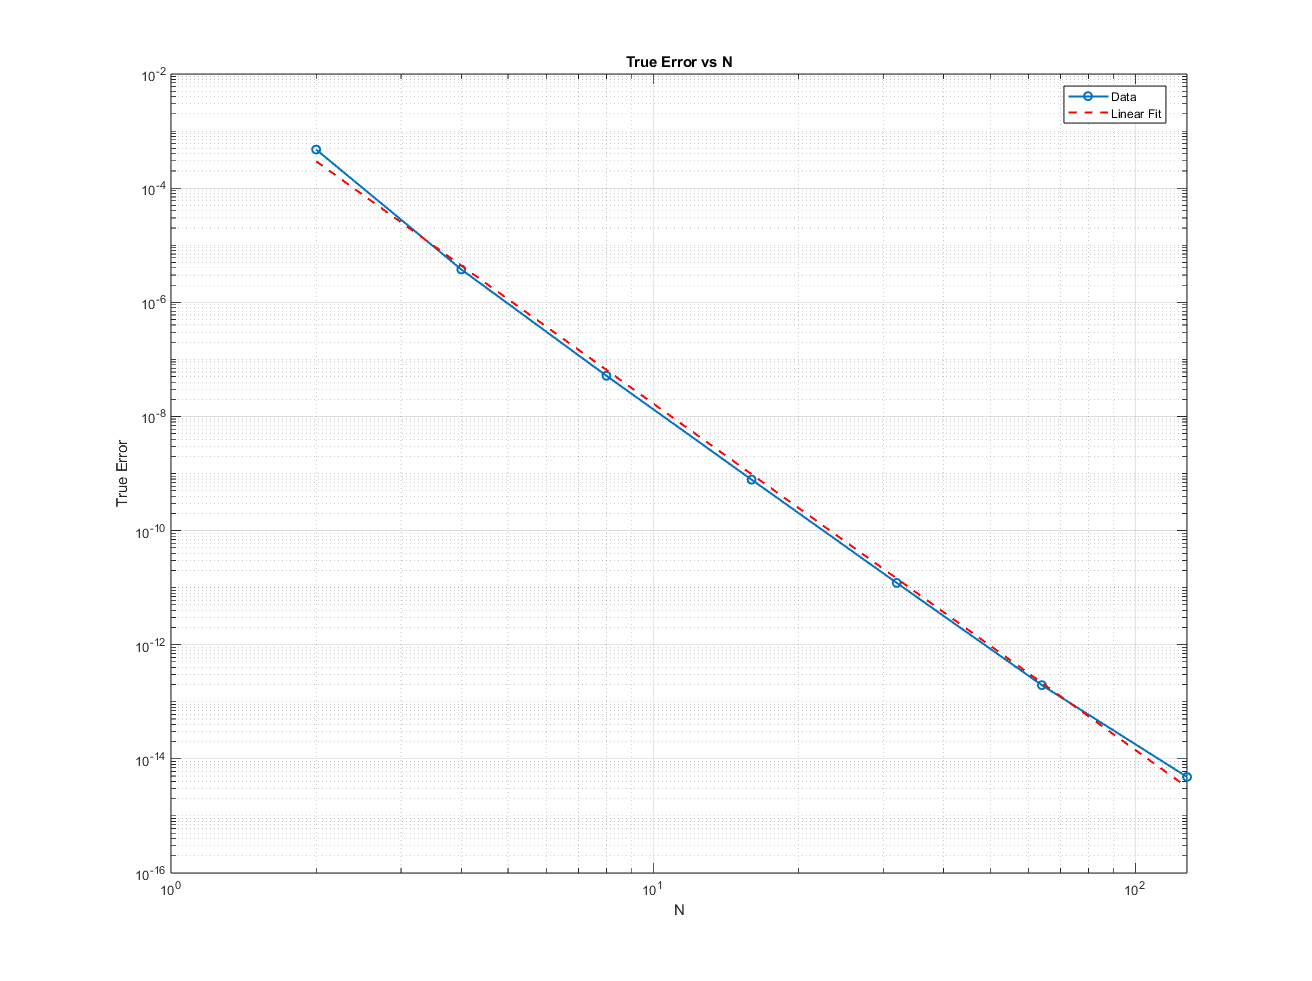
\includegraphics[width=1\textwidth]{Q2-plot2.png}
    \caption{True Error vs $N$ for $\sin(x^3) \cos(x)$}
    \label{fig:sinx3cosx}
\end{figure}

The slope of the plotted curve on figure 2 is -6.07. Indicating the error doesn't converges slower with varying number of segments compared to the part b. However, true error is also bigger for part c.

